\chapter{Methodology}
\label{chap:met}
In this chapter I provide description of improvement of current metrics. As I pointed in introduction I divided metrics on two types: distance metrics and score metrics. In distance metrics I change three aspects: feature extractor, distance computer and dataset on which metric is computing. In score metrics I change two aspects: feature extractor, dataset for finetuning of feature extractor. In this chapter I will describe the experiments I will conduct to evaluate the validity of the metric. Also I will provide new metric which would be somewhere in between distance metrics and score metrics.
\section{Distance metrics}
As I described in literature review FID consist of InceptionV3 as feature extractor and Fréchet Distance as distance metric which compute distance between two distributions: real images and generated images. So, I generalized diagram of FID from literature review chapter to distance metric at the Figure \ref{fig:DistanceMetric}:
\begin{figure}[hbt]
\centering
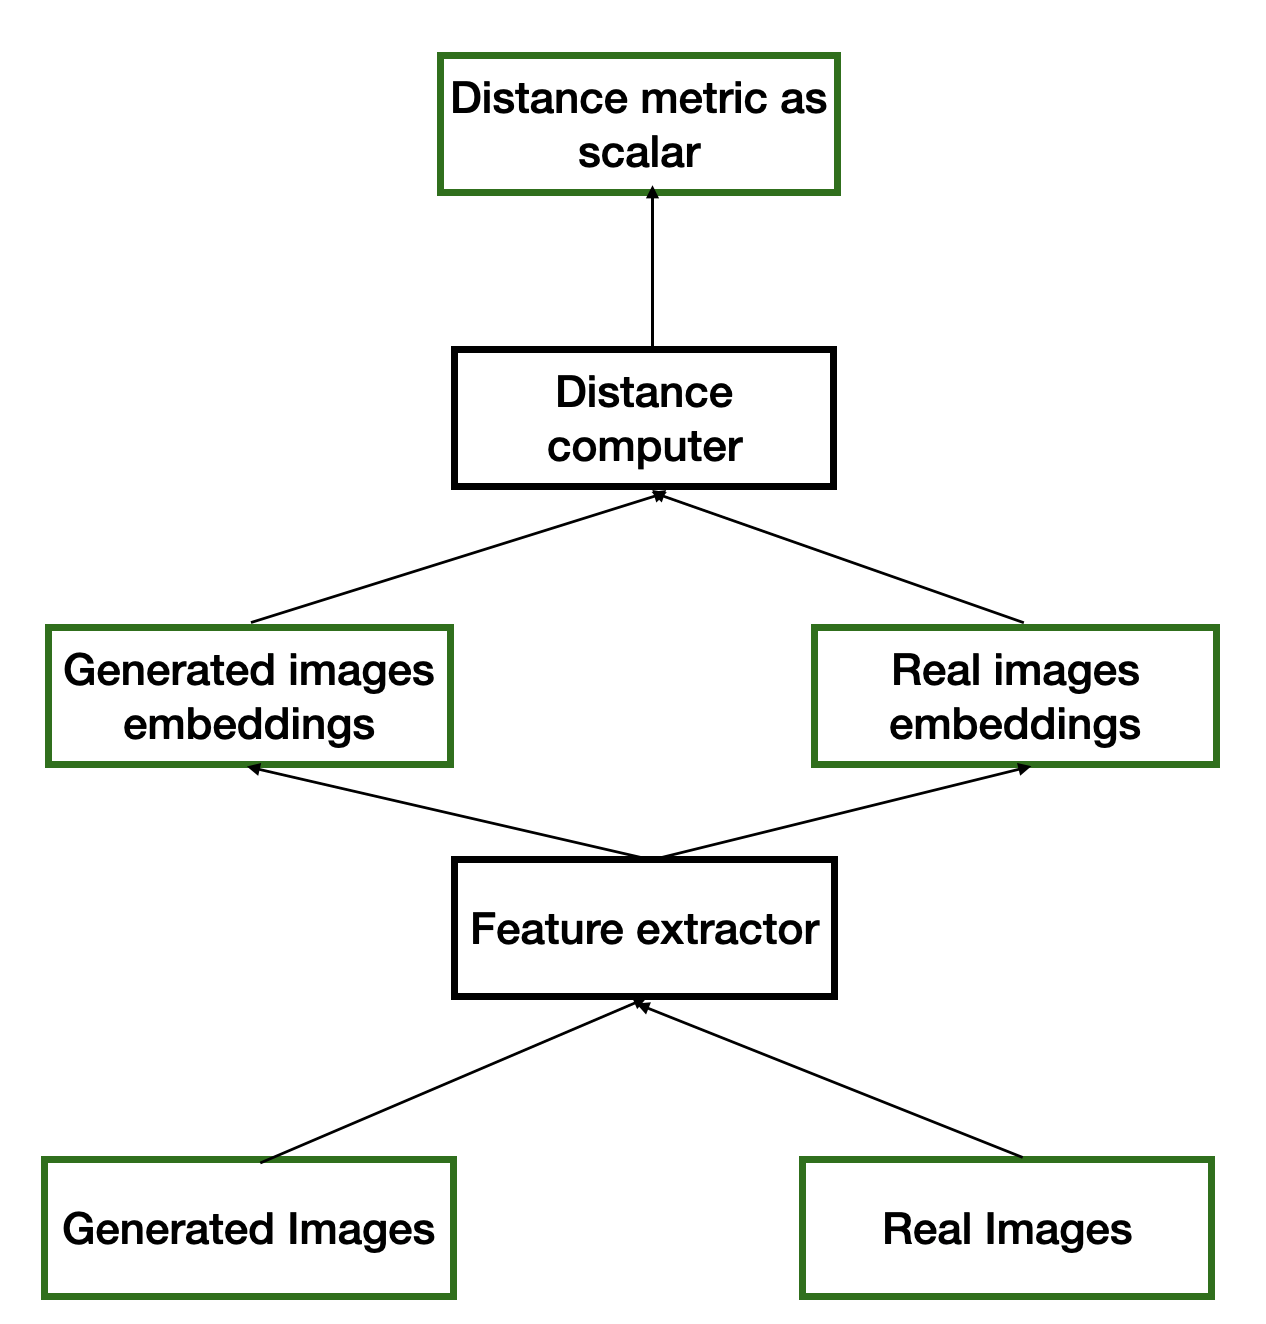
\includegraphics[width=8cm, height=10cm]{figs/distance_metric.png}
\caption{The diagram of distance metric}
\label{fig:DistanceMetric}
\end{figure}


The diagram shows that there are two components in the metric that can be changed: feature extractor - a model with which we extract features (embeddings) from images and distance computer - a formula that calculates the distance between embeddings of real and generated images. Actually, there's also a third component, which is a dataset of real pictures and prompts. Prompts are used to generate pictures, and real pictures are used to calculate metrics.

\subsection{Feature extractor}
As feature extractor I use three models: InceptionV3, image encoder from CLIP architecture and DINOv2. DINOv2 and CLIP are a self supervised models. I sue self supervised models due to they better adaptability to new domains, better solving zero-shot problems and richer extracted features. I will not describe CLIP architecture here because I have already described it in the literature review chapter.
\subsubsection{DINOv2}
DINO\cite{DINO} develops the Siamese network approach with a momentum encoder update of one of the branches and introduces a view of this process as Knowledge distilation. 

Accordingly, the distilation takes place from teacher to student through cross-entropy of probability distributions. The student's weights are updated through the backprop mechanism, while the teacher's weights are updated through a moving average of the student's weights.

Mathilde Caron et al. \cite{DINO} replace BatchNorm with 2 procedures - centering and sharpening, which is essentially the same normalization, only the shift parameter in centering is updated via moving average. The authors describe the effect as follows: "centering prevents one dimension to dominate but encourages collapse to the uniform distribution, while the sharpening has the opposite effect"\cite[p.4]{DINO}. Mathilde Caron et al. \cite{DINO} use multicrop and show that increasing the number of local image patches improves the quality.
They also use this method to train the Transformer (ViT) and find an interesting effect - right out of the box, the network starts segmenting the image without any partitioning. And it does it better than supervised learning. I provide diagram of DINO model at the Figure~\ref{fig:DINO_dian}.
\begin{figure}[hbt]
\centering
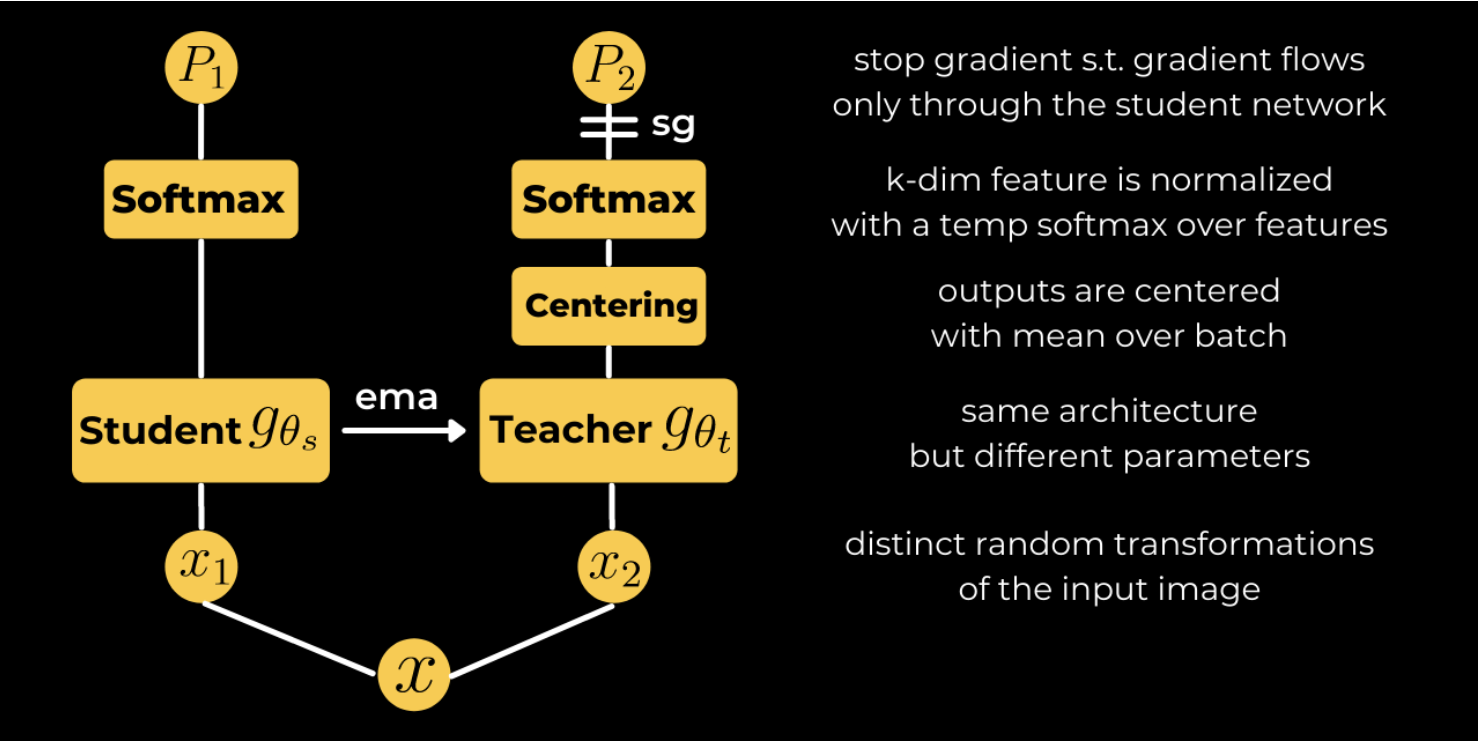
\includegraphics[width=15cm, height=10cm]{figs/DINO_diag.png}
\caption{Diagram of DINO}
\label{fig:DINO_dian}
\end{figure}

Also, I provide images and segmentation maps generated by DINO model and original images at the Figure~\ref{fig:DINO_seg_map}. I take it from original paper\cite{DINO}.
The figure shows how clearly DINO makes a segmentation map of the picture. DINOv2 is able to do higher-quality segmentation due to more careful and longer training.
\begin{figure}[hbt]
\centering
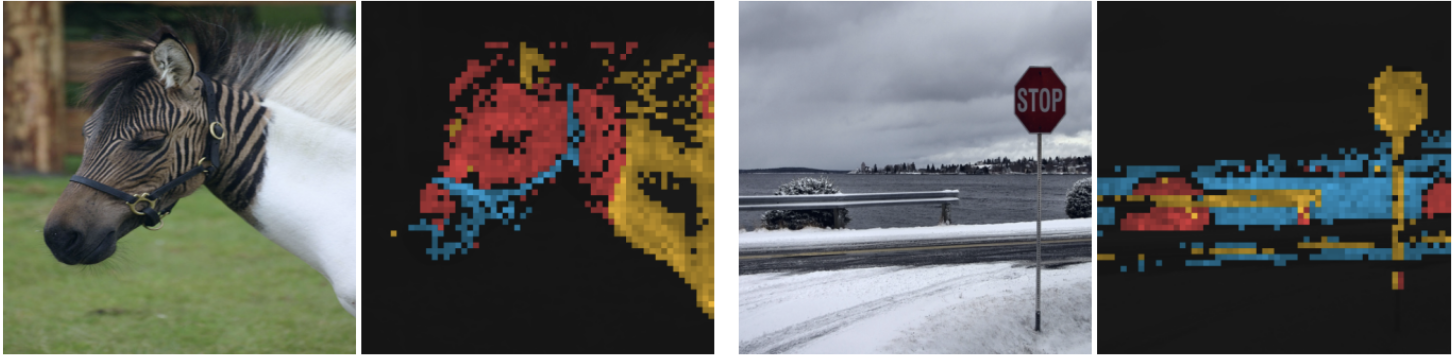
\includegraphics[width=15cm, height=5cm]{figs/DINO_seg_map.png}
\caption{Segmentation maps generated by DINO model and original images\cite{DINO}}
\label{fig:DINO_seg_map}
\end{figure}

DINOv2 is an improved version of DINO. DINOv2 generates not one feature for all images, but one feature for each 14*14 pixel square. This gives much more understanding of what is going on, and solves some of the CLIP problems.

\subsection{Distance computer}
As distance computer I choose tho methods: fréchet distance(FD) and kernel distance(KD). Kernel distance is also called maximum mean discrepancy(MMD). I choose FD due to it is standard distance computer function in such metric as FID and KD due to it is promising method which does not make assumtion about normality of distribution in contrast to FD.
\subsubsection{Kernel Distance}
In the following under kernel distance(KD) and maximum mean discrepancy I will have the same thing. I got the idea of using KD as a formula for calculating the distance between distributions from an article that uses KD together with embeddings from CLIP\cite{KD_CLIP}.

KD is described using the following formula:
\begin{equation}
dist^2(P,Q)=\mathbb{E}_{x,x'}[k(x,x')] + \mathbb{E}_{y,y'}[k(y,y')] -2\mathbb{E}_{x,y}[k(x,y)]
\end{equation}
Sadeep et al. provide information:"$x$ and $x'$ are independently distributed by $P$ and $y$ and $y'$ are independently distributed by $Q$"\cite[p.5]{KD_CLIP}.
If we have two datasets, $X={x_1,x_2,...,x_m}$ sampled from $P$ and $Y={y_1,y_2,...,y_m}$ sampled from $Q$, then unbiased estimator will be
\begin{equation}
\begin{split}
dist^2(X,Y)=\frac{1}{m(m-1)}\sum_{i=1}^{m}\sum_{j\neq i}^{m}k(x_i,x_j)\\+\frac{1}{n(n-1)}\sum_{i=1}^{n}\sum_{j\neq i}^{n}k(y_i,y_j)\\-\frac{2}{mn}\sum_{i=1}^{m}\sum_{j=1}^{n}k(x_i,y_j)
\end{split}
\end{equation}
As the kernel I use the Gaussian kernel $k(x,y)=-\frac{||x-y||^2}{2\sigma^2}$. Advantages of KD over the FD are:
\begin{itemize}
    \item KD is distribution-free meaning that it does not require a normal distribution of images as FD.
    \item KD is unbiased.
    \item KD is efficient from a computational point of view, since it does not require the computation of large matric as FD requires.
\end{itemize}
\subsection{Dataset for evaluation}
The dataset is very important for calculating the metric, as the actual images from the dataset determine what we should be aiming for with the generative model. I chose two datasets for my experiments:
\begin{enumerate}
    \item COCO with captions\cite{COCODataset}. it is 41 thousand real images. This is a standard dataset that is used to evaluate other metrics in other articles\cite{KD_CLIP}. In Figure\ref{fig:COCO_examples} it's possible to see that these are real images.
    \item MJHJ30K\cite{MJHQ30K}. This is a dataset of high-quality images generated with Midjourney with 10 common categories, each category with 3K samples. The difference of this dataset from COCO is that it contains not real, but more beautiful and aesthetic images. That is, it is better to use it if the model should generate aesthetic images similar to those generated by Midjourney. In Figure\ref{fig:MJHQ30k_examples} it's possible to see that the images are substantially different from those in COCO. The obvious differences are that the images in MJHQ30k are more aesthetically pleasing, more contrast and detailed.
\end{enumerate}

\begin{figure}[hbt]
\centering
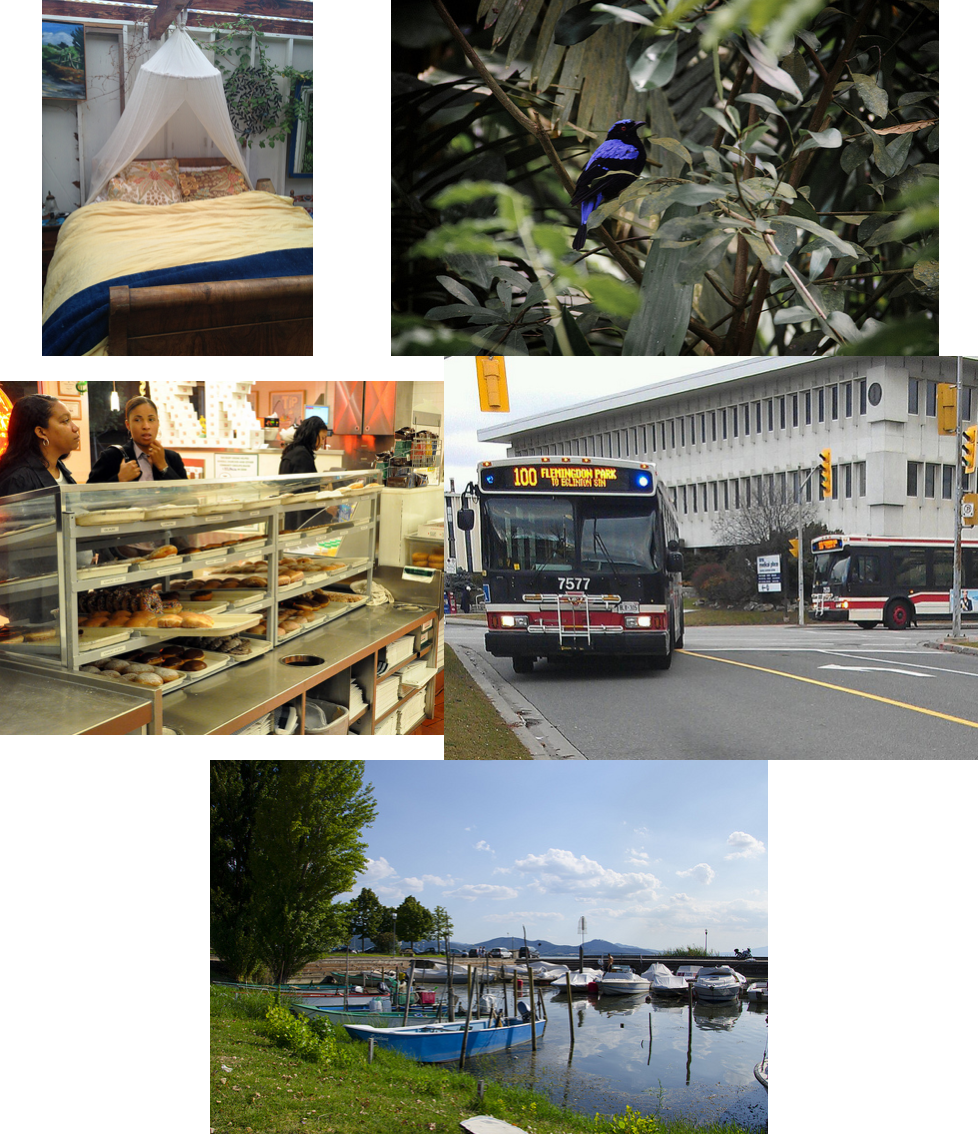
\includegraphics[width=7cm, height=10cm]{figs/coco_examples.png}
\caption{Images from COCO dataset with 41K real images}
\label{fig:COCO_examples}
\end{figure}

\begin{figure}[hbt]
\centering
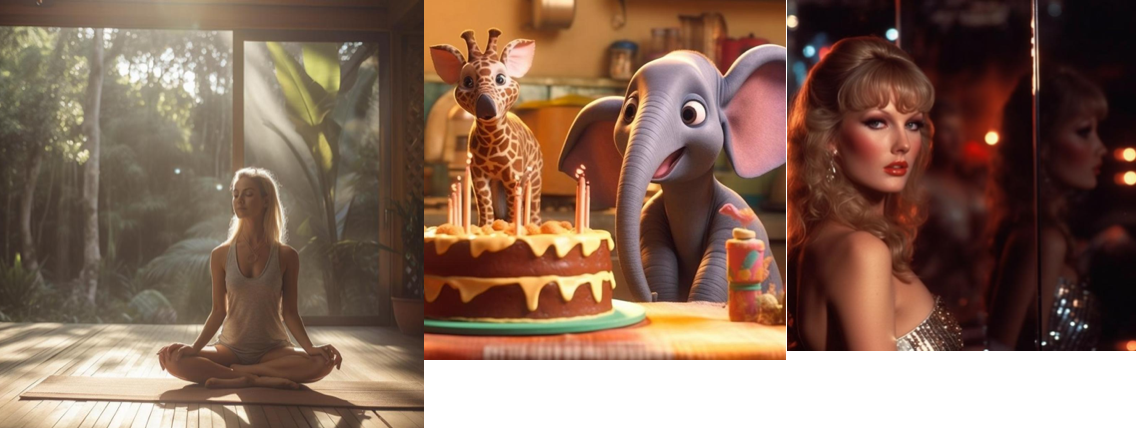
\includegraphics[width=12cm, height=5cm]{figs/mjhq30k_examples.png}
\caption{Images from MJHQ30K dataset with 30K generated by Midjourney and filted images}
\label{fig:MJHQ30k_examples}
\end{figure}

\subsection{Summary}
In conclusion, I chose three different models as feature extractor, two methods as distance computer and two datasets. This adds up to a total of 12 different metrics.\\
\begin{table}[h]
\centering
\begin{tabularx}{0.8\textwidth} { 
  | >{\centering\arraybackslash}X 
  | >{\centering\arraybackslash}X 
  | >{\centering\arraybackslash}X | }
 \hline
  & Kernel Distance(KD) & Fréchet Distance(FD) \\
 \hline
 InceptionV3  & KID  & FID  \\
 \hline
 CLIP  & KD\_CLIP  & FD\_CLIP  \\
\hline
 DINOv2  & KD\_DINOv2  & FD\_DINOv2  \\
\hline
\end{tabularx}
\caption{Distance metrics}
\label{tab:distance_metrics}
\end{table}
\section{Score metrics}
Idea behind each score metric is to extract
features(embeddings) from prompt and generated image and calculate simmula-
rity between two embeddings. Resulting scalar will be result of the metric. For the results of such a metric to be correct, it is necessary to be sure that the embeddings of the image and the prompt are in the same vector space. This property is represented by CLIP\cite{CLIP} and its variants such as BLIP\cite{BLIP}. The diagram of score metric is shown at the Figure\ref{fig:Score_metric}.
\begin{figure}[hbt]
\centering
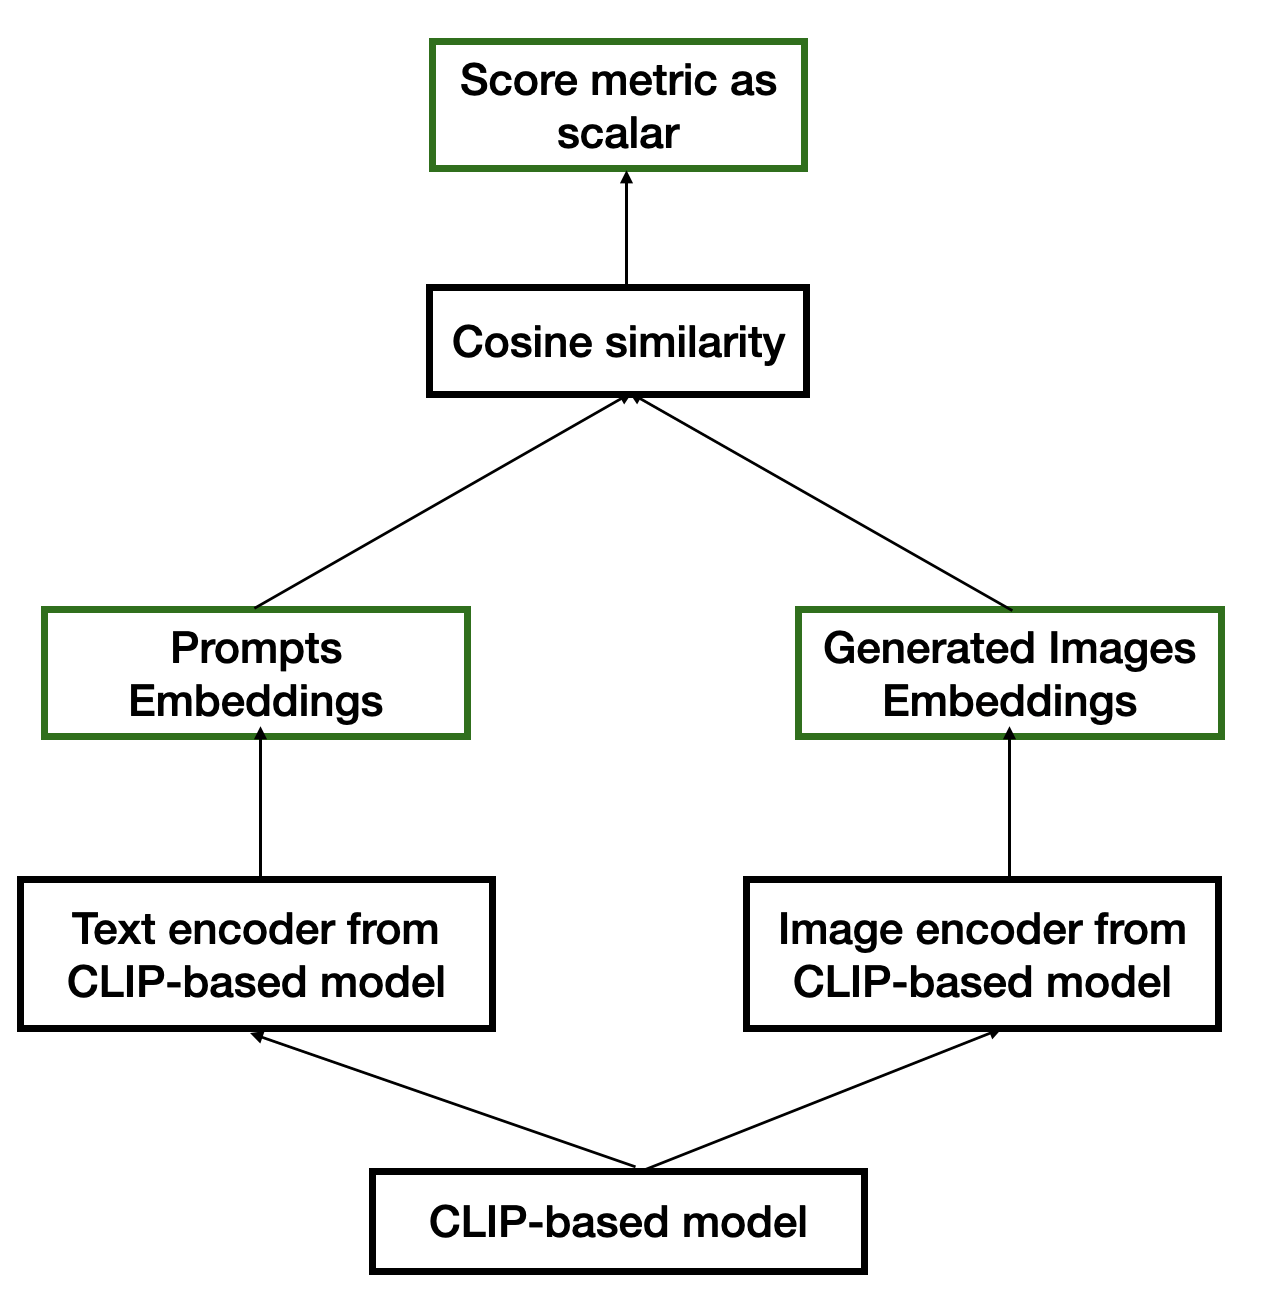
\includegraphics[width=8cm, height=10cm]{figs/score_metric.png}
\caption{Diagram of score metric}
\label{fig:Score_metric}
\end{figure}
I'll be using the following score metrics:
\begin{enumerate}
    \item ClPPscore\cite{CLIPScore} - standard metric.
    \item MCLIPScore - CLIPSore but with MCLIP instead CLIP.
    \item ImageReward\cite{Image_reward}.
    \item HPSv2\cite{HPSv2}.
\end{enumerate}
\subsection{MCLIPScore}
Idea is the same as in CLIPScore which I descibed in literature review chapter, but MCLIP is used instead of CLIP.

Unlike CLIP, which learns and works predominantly with English, MLIP learns and is able to interpret texts in different languages, which improves its applicability globally.
\subsection{ImageReward}
Idea of ImageReward\cite{Image_reward} is to use BLIP architecture with modification and make new dataset for finetuning. Jiazheng et al.\cite{Image_reward} take the features from prompt and image using BLIP, combine them using Cross-Attention and using linear layer make a scalar to get the score.
\subsubsection{BLIP}
The main goal of BLIP (Bootstrapped Language Image Pretraining) is to improve the model's ability to interact between language and visual content.


While CLIP is trained using contrastive learning, which aims at converging vector representations of images and corresponding textual descriptions, BLIP introduces additional tactical strategies, such as self-distillation, to improve the stability of learning and the quality of the representations generated by the model. Self-distillation is a technique where knowledge from one part of the model is transferred to another part of the model, improving its overall performance and generalization ability.
\subsubsection{ImageReward Dataset}
Jiazheng et al. used DiffusionDB: a prompt and image database created with Stable Diffusion. DiffusionDB stores 1.8M data which is too much, so certain prompts are selected using the following algorithm:
\begin{enumerate}
    \item Prompts are encoded using Sentence-BERT and KNN is constructed with cosine similarity as distance.
    \item Score of each vertex is formed as the number of neighbors which are not selected.
    \item Vertices are selected based on score and then score is recalculated.
    \item Since the complexity is quadratic, the dataset is divided into 100 sets (20k prompts in each set) and 100 prompts are selected in each set -> 10k diverse prompts in the end.
\end{enumerate}
Further, to finetune on this dataset the model it was necessary to assign to each pair of generated image-prompt some score. For this purpose, people were involved who evaluated pairs on a 7-ball scale of aesthetics, relevance and defectiveness.

ImageReward model is funetuned using the following formula:
\begin{equation}
loss(\theta)=-\mathbb{E}[log(\sigma(f_\theta(T,x_i) - f_\theta(T,x_j)))]
\end{equation}
where $T$ is a prompt and $x_i$ is a image that better then $x_j$ image.
\subsection{HPSv2}
The idea behind HPSv2\cite{HPSv2} is to make your own dataset and finetune CLIP on it.
\subsubsection{Dataset collecting}
Prompts are taken from two datasets “COCO Captions” and “DiffusionDB” cleaned with chatGPT.

Xiaoshi et al. take different model patterns and generate a picture of each pattern for each prompt. Also for the prompts from “COCO Captions” real pictures are taken\cite{HPSv2}.

The test data is 400 groups. Of them 300 groups from DuffusionDB generated by 9 models and 100 groups from COCO Captions generated by 9 models and plus one real picture from COCO Captions. Total 10 anonators per group: 300 * (9 * 8 / 2) * 10 + 100 * (10 * 9 / 2) * 10 = 300 * 360 + 45000 = 108000 + 45000 = 153000 binary comparisons.


Train data is 107,515 groups. Each group is 4 pictures(coherent or real) and one anotator. 28,172 groups from COCO Captions the rest from DiffusionDB.

\subsubsection{Finetune process}
HPSv2 takes ViT-H/14 CLIP and fine-tune using the collected dataset. Train instance is two pictures $x_1$, $x_2$ of one prompt $p$ and $y=[1,0]$ if $x_1$ is better than $x_2$. CLIP score is counted with temperature(trained parameter):
\begin{equation}
s_\theta(p,x)=\frac{Enc_{txt}(p)*Enc_{img}(x)}{\tau}
\end{equation}
Predicted preference is calculated as:
\begin{equation}
\hat{y_i}=\frac{exp(s_\theta(p,x_i))}{\sum_{j=1}^{2}exp(s_\theta(p,x_j))}
\end{equation}
Then the training loss is:
\begin{equation}
L_{pref}=\sum_{j=1}^{2}y_i(log(y_i)-log(\hat{y_j}))
\end{equation}
Only the last 20 layers of image encoder and 11 layers of text encoder are trained.
\section{Human evaluation}
To determine a person's judgement I by themselves marked up mini datasets consisting of 300 samples, where a sample consists of a real picture, a prompt, and a generated picture. Such mini dataset was for each model used and for each dataset.

\section{Cosine similarity with DINOv2 features}
The problem with distance metrics is that they do not take into account in any way the information that the generated image and the real one refer to the same propmt. The problem with score metric is that it does not take into account the aesthetics of the picture as the metric simply does not include the aesthetic (real) picture to be based on.

I propose a method of computing metric that can anihilize both of these disadvantages. The idea of my metric is to take a feature extractor for each pair, extract the embeddings of the real and generated images and use cosine simularity to get the similarity of the two embeddings. To get a score for a dataset the arithmetic mean for each pair from the dataset is taken. The scheme of this metric would look like this:
\begin{figure}[hbt]
\centering
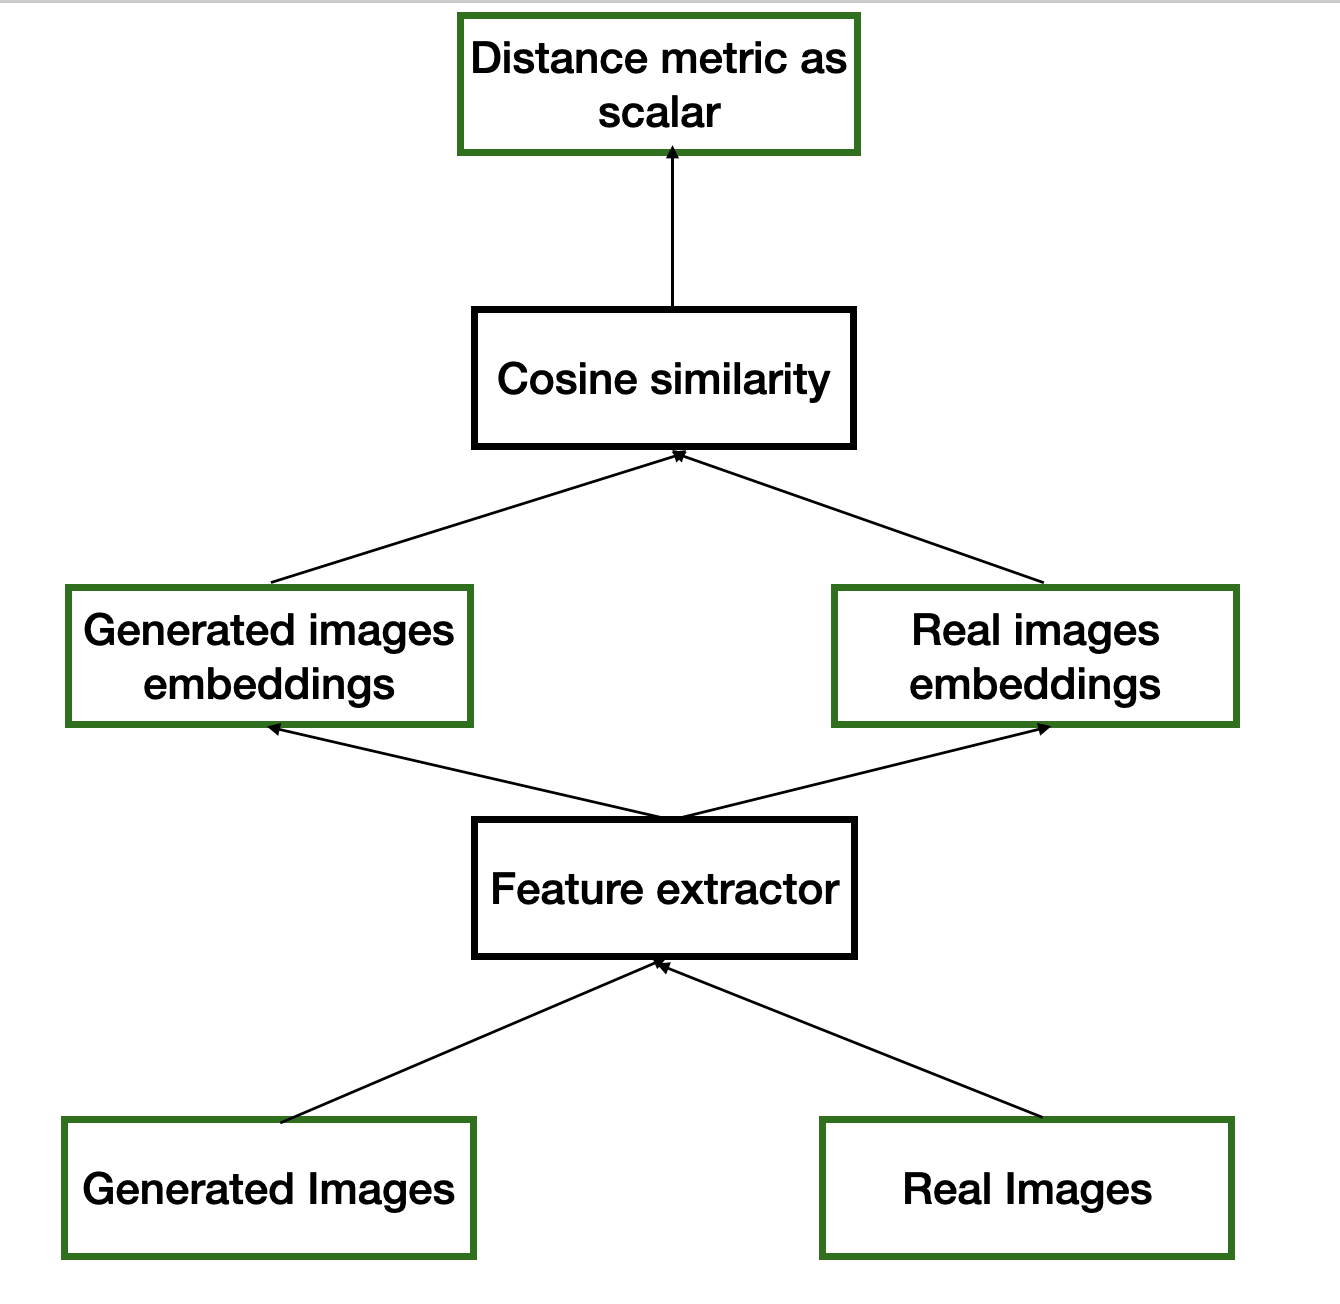
\includegraphics[width=8cm, height=10cm]{figs/cos_clip.png}
\caption{Diagram of my own metric, COS\_DINOv2}
\label{fig:cos_dinov2_diagram}
\end{figure}
It is possible to notice that the diagram is very similar to the distance metric. But it is important to note that to calculate distance in distance metric, some qualities are taken from embedding datasets, for example, mean and variance for FD or Gaussian kernel for KD. While in my method distance is calculated on embeddings for each pair directly.

I will use DINOv2 as a feature extractor in the experiments chapter in the future. I call such a metric COS\_DINOv2.